\subsection{Motivation}

\par Cette représentation géométrique s'éloigne des représentations précédentes pour plusieurs raisons. Premièrement, elle s'inscrit dans l'idée de formuler des problèmes plus simples (REF MOD DIST REL) suite à l'échec des modèles utilisant les représentations précédentes (REF MOD DELTA DIST). Pour cette raison, nous n'allons plus chercher à représenter des molécules complètes mais uniquement des liaisons covalentes\footnote{Une liaison covalente est une liaison chimique dans laquelle deux atomes se partagent deux électrons (un électron chacun ou deux électrons venant du même atome) d'une de leurs couches externes afin de former un doublet d'électrons liant les deux atomes. (Wikipédia)} entre des paires d'atomes au sein des molécules. Cette représentation doit contenir des informations permettant aux modèles l'utilisant de prédire la longueur de la liaison représentée, sans bien-sûr l'enregistrer directement.\\
En second lieu, la contrainte majeure de la nécessité d'être capable de reconstruire la matrice des coordonnées atomiques à l'issue des prédictions des modèles utilisant cette représentation disparaît. En effet, si l'on peut imaginer des représentations similaires (REF REPR ANGLES) et un assemblage de modèles (REF MODULES) qui permettraient de reconstruire la matrice de coordonnées atomiques d'une molécule convergée (REF DEF CONVERG), il s'agit d'objectifs hors de notre portée pour le moment, notre objectif étant dans un premier temps de valider notre capacité à prédire des géométries moléculaires.

\subsection{Classes positionnelles}
\par La longueur d'une liaison covalente entre deux atomes dépend du type des atomes formant la liaison, mais également de l'influence des atomes au voisinage de la liaison, qui dépend de leur position relativement aux atomes de la liaison. C'est pour cette raison que nous formalisons la notion de classe positionnelle qui va représenter de quel « côté » de la liaison chaque atome se trouve. Les atomes peuvent donc être « à gauche », « au centre » ou « à droite » de la liaison.\\
Formellement, on compare la position des atomes aux deux plans normaux à la liaison et passant par les atomes de la liaison. Si un atome est entre les deux plans, il est de classe « centre », sinon il est de classe « gauche » ou « droite » en fonction du plan dont il est le plus proche. Puisque l'on se place dans le repère relatif de la liaison et qu'il n'y existe pas de notion absolue de gauche ou de droite, ces deux classes sont interchangeables à condition que les atomes appartenant à une classe soient tous à distance minimale du même plan.

\vspace{1cm}

\begin{figure}[!h]
	\centering
	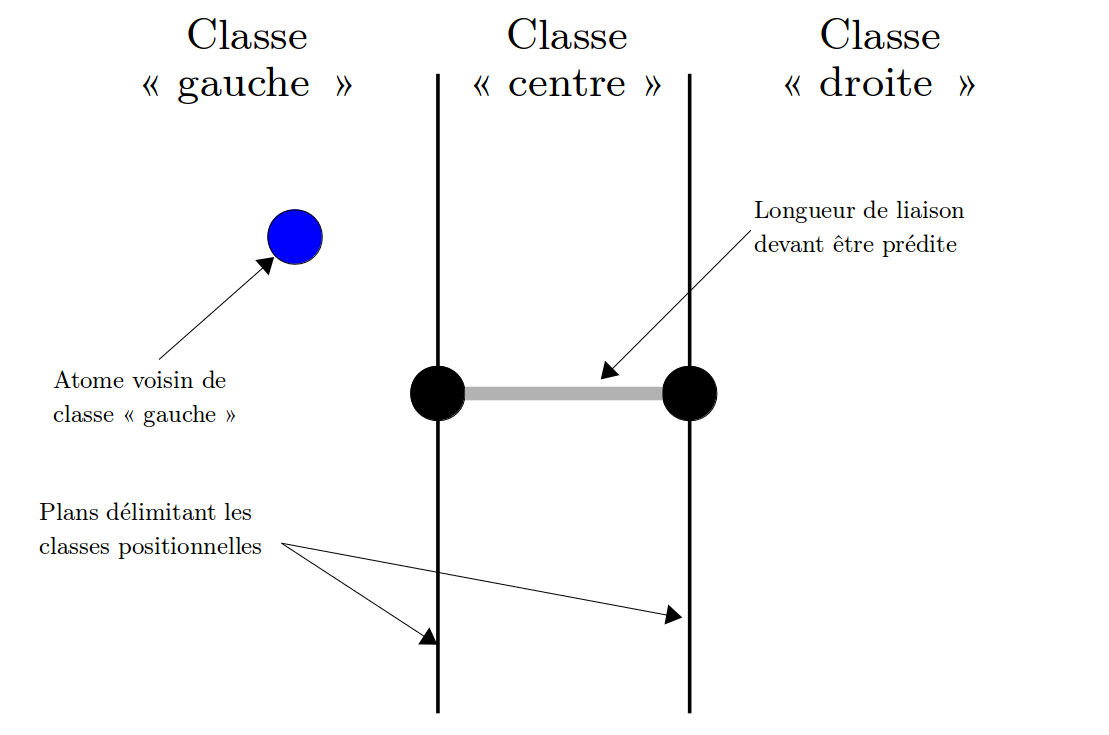
\includegraphics[scale=0.27]{images/classes_pos.png}
	\caption{Classes positionnelles au voisinage d'une liaison covalente}
\end{figure}

\subsection{Distances aux atomes de la liaison}
\par L'influence des atomes au voisinage de la liaison dépend également de leur distance à chacun des deux atomes de la liaison. Plus l'atome voisin est près, plus son influence est forte. C'est pourquoi notre représentation contient également cette information. \\
En fonction des modèles qui l'utilisent, on va éventuellement appliquer une fonction à ces distances, afin de mieux rendre compte de l'influence réelle des atomes au voisinage. Si les réseaux de neurones sont capables d'approximer ces fonctions lors de l'apprentissage, d'autres modèles comme les SVM (REF SVM) ne le sont pas et l'application de ces fonctions est donc nécessaire pour espérer obtenir de bons résultats. Ces fonctions sont les suivantes.\\

\begin{itemize}
\item{Fonction identité : distance brute}
\item{Fonction inverse : influence inversement proportionnelle à la distance, relation d'ordre identique à la réalité chimique.}
\item{Fonction inverse du carré : influence inversement proportionnelle au carré de la distance, relation d'ordre identique à la réalité chimique et rend mieux compte de l'influence réelle des atomes qui est liée à la loi de Coulomb\footnote{https://fr.wikipedia.org/wiki/Loi\_de\_Coulomb\_(électrostatique)} en $\frac{1}{d^2}$.}
\end{itemize}

\vspace{0.4cm}

\par Notons qu'aucune de ces fonctions ne représente parfaitement l'influence des atomes en fonction de leur distance, elles permettent cependant de s'approcher de la réalité.

\vspace{1cm}

\begin{figure}[!h]
	\centering
	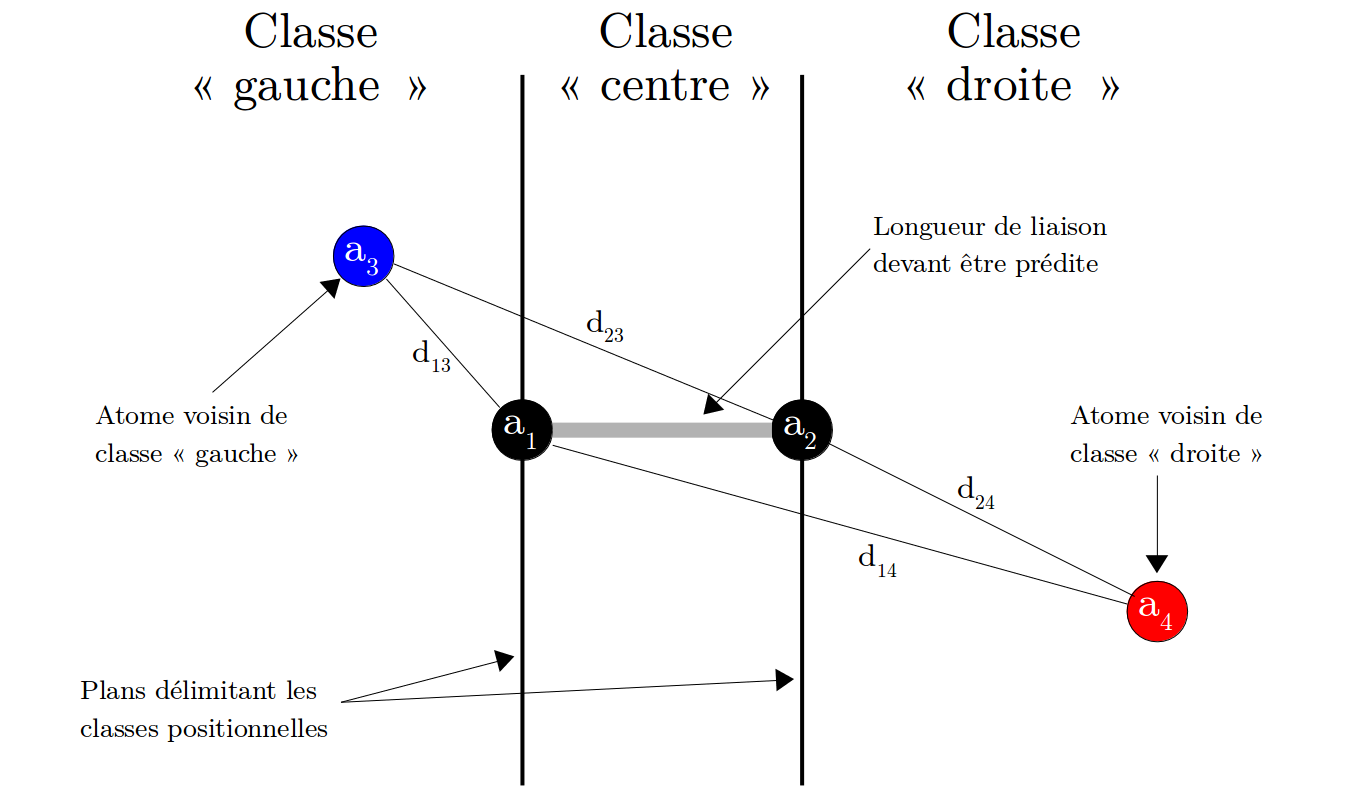
\includegraphics[scale=0.28]{images/classes_pos_2.png}
	\caption{Distances des atomes à chacun des atomes de la liaison covalente}
\end{figure}


\subsection{Restriction au voisinage le plus proche}
\par L'influence des atomes au voisinage de la liaison étant inversement proportionnelle à leur distances aux atomes de la liaison, elle décroît rapidement lorsque l'on s'éloigne de la liaison. L'influence des atomes n'étant pas au voisinage direct est ainsi négligeable. Dans le but de ne pas saturer l'entrée des modèles d'information inutile, nous n'enregistrons alors que les informations (classes positionnelles, distances et autres informations non géométriques spécifiques aux différents modèles) concernant les atomes au voisinage proche de la liaison. Formellement, nous enregistrons ces informations pour les atomes dont la distance à au moins un des atomes de la liaison est inférieure à un seuil $\epsilon$  donné.\\

\vspace{1cm}

\begin{figure}[!h]
	\centering
	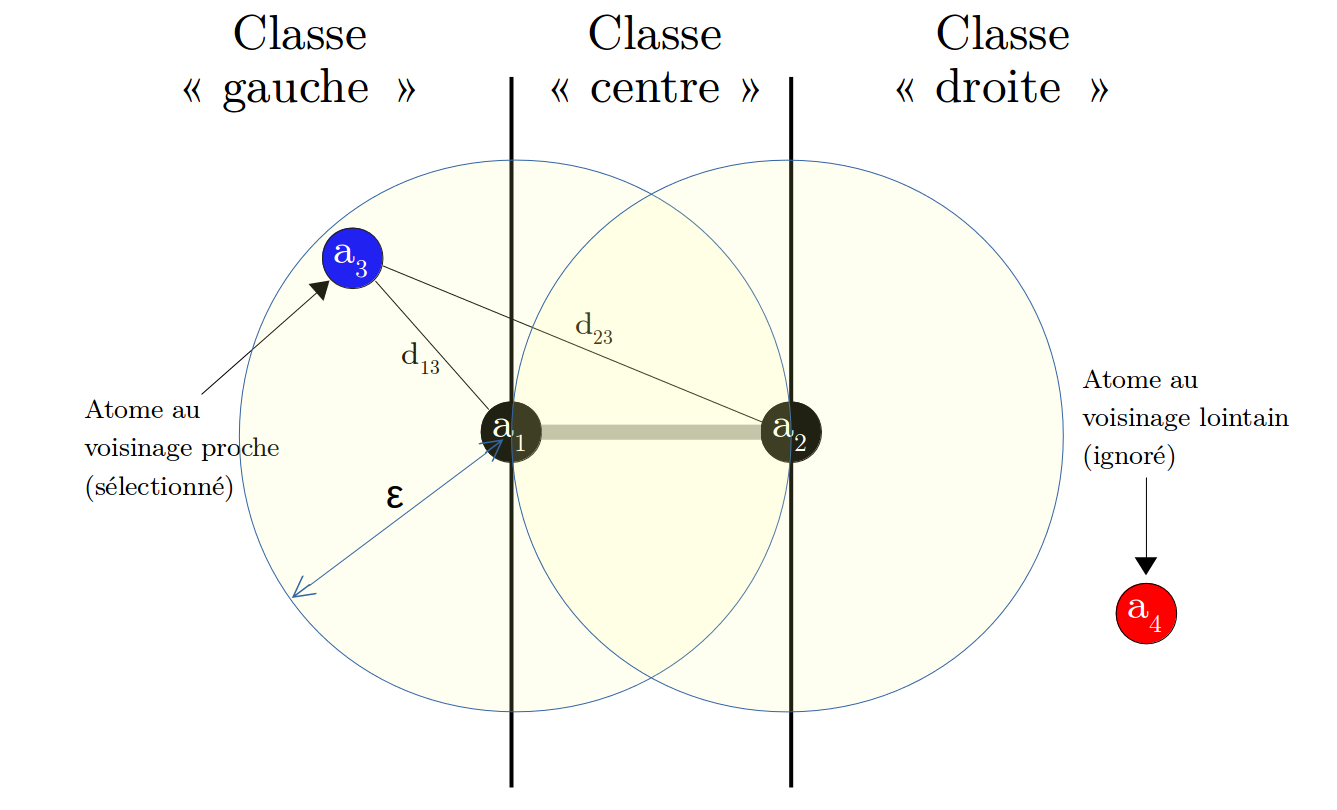
\includegraphics[scale=0.28]{images/classes_pos_3.png}
	\caption{Sélection des atomes au voisinage le plus proche}
\end{figure}

\par Un autre avantage de cette sélection est qu'il existe des molécules aux géométries particulières (repliées) telles que des atomes au voisinage d'une liaison ont très peu d'influence sur sa longueur (ne forment aucune liaison covalente avec les deux atomes de la liaison), et dont la proximité va induire les modèles en erreur. La sélection des atomes au voisinage le plus proche de la liaison avec un seuil $\epsilon$ bien choisi va permettre de résoudre ces problèmes.

\begin{figure}[!h]
	\centering
	
	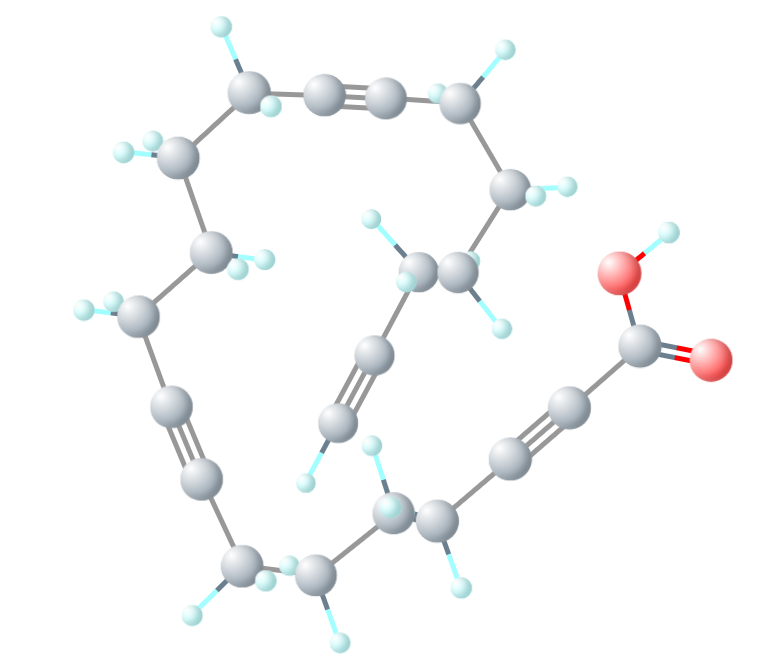
\includegraphics[scale=0.25]{images/mol_repliee.png}
	\caption{Exemple de molécule repliée (CID Pubchem 328310)}
\end{figure}